\documentclass[
  outputdir=build,
  chapterstyle=cn,
  colorscheme=Simple,
  fontset=tech,
  code=false
]{Hypo-Note}

\usepackage{graphicx}
\usepackage{booktabs}
\usepackage{longtable}
\usepackage{tabularray}
\UseTblrLibrary{booktabs}
\usepackage{tabularx}
\usepackage{colortbl}
\usepackage{array}
\usepackage{enumitem}
\usepackage{tikz}
\usepackage{pgfplots}
\usepackage{float}
\usepackage{caption}
\usepackage{listings}
\usepackage{multicol}
\usetikzlibrary{arrows.meta,positioning,fit,matrix,trees}
\pgfplotsset{compat=1.18}
\graphicspath{{assets/}{figures/}{vendor/Hypoxanthine-LaTeX/assets/}}
\definecolor{HWGray}{HTML}{6B7280}
\definecolor{HWBlue}{HTML}{7FAEDB}
\definecolor{HWGold}{HTML}{E8D89D}
\newcommand{\code}[1]{{\small\texttt{\detokenize{#1}}}}

\HypoNoteSetup{
  title={Hypo-Workflow：面向 AI Agent 的 Harness Engineering 实践},
  subtitle={从个人 AI Coding 经验到可规划、可恢复、可审计的工程工作流},
  author={Hypo-Workflow Project Draft},
  affiliation={Technical Report for Lab Presentation},
  date={2026-05-01}
}

\HypoCoverSetup{
  style=academic,
  background=sidebar,
  color=HypoSimple02OnlyBlue,
  subject={Harness Engineering / Technical Report},
  image={assets/gpt-image/cover-harness-engineering.png}
}

\lstset{
  basicstyle=\ttfamily\small,
  frame=single,
  breaklines=true,
  columns=fullflexible,
  keepspaces=true,
  backgroundcolor=\color{HypoSurface}
}

\title{Hypo-Workflow：面向 AI Agent 的 Harness Engineering 实践}
\author{Hypo-Workflow Project Draft}
\date{2026-05-01}

\begin{document}

\makecover
\frontmatter
\tableofcontents
\mainmatter

\chapter{引言：从个人 AI 使用经验到工程问题}

\section{问题不是“AI 会不会写代码”，而是“AI 能不能持续做工程”}

这份报告的目标，不是介绍一个新的 prompt 技巧，也不是宣传某个单次对话式开发体验有多惊艳。真正的问题是：当 AI 从“补一段代码”升级为“参与一个跨文件、跨会话、可交付、需要验收和维护的工程过程”时，原有工具往往会迅速暴露结构性缺陷。

作者对 AI Coding 的理解并不是从理论出发，而是从一条非常具体的使用路径出发。最早的阶段主要依赖网页端 GPT / Gemini，或者在 Cherry Studio 中调用 DeepSeek 模型。这一阶段的工具当然能回答编程问题，但无法直接读取完整代码库，也无法稳定持有项目约束。任何一次稍微复杂一点的任务，都要求用户反复补充背景、接口、风格、目录结构和期望行为。表面上是在“问模型”，实际上是在做人肉状态同步。

接下来转向 GitHub Copilot。Copilot 的优势很明确：局部补全很强，续写代码的即时反馈也很好。但它的弱点也同样明确：规划能力有限，对代码库整体约束的感知并不稳定，尤其在多文件协作、跨模块重构和长期风格统一上，仍然需要大量人工干预。这个阶段，作者一度通过堆叠人工 prompt 和外部文档的方式，让 AI 维护 \texttt{CHANGELOG}、\texttt{FEATURES}、版本摘要等文件，并在 Hypo-LaTeX 一类项目上获得初步成效。但这并不意味着问题解决了，只是说明“人可以靠大量手工约束把结果拉回正确轨道”。

随后尝试过 AntiGravity。与更早的工具相比，它的“自动化感”更强，但这种强更多体现在表层交互，而不是工程可靠性上。自动化越多，反而越需要可追踪、可验证、可纠偏的约束系统；否则，错误会被包裹在更漂亮的流程里。AntiGravity 在需求表达空间、行为可控性和验证闭环上的不足，恰好加深了这种认识：自动化本身不是答案，可验证的自动化才是。

寒假开始大规模使用 Claude Code。这是一个真正的拐点。对话式实现能力、上下文组织和中等规模任务的完成度都比前述工具高得多，首次让“Agent 像是在认真协作写代码”这件事变得可信。但新的问题也浮现出来：即使模型足够聪明，用户仍然需要反复粘贴类似的约束，例如输出语言、计划先行、不要越权改文件、修改后要补测试、保持文档同步、按某种风格回答。这说明智力的提升并不自动带来行为固化。

进一步地，作者又接触到 Skills 和类似 Superpowers 的“先计划后做”思路。这一阶段非常关键，因为它第一次把“做之前先拆清楚”正式纳入工作流，而不仅仅是临场提醒。问题在于，这种规划往往只在单次任务里表现优秀；一旦项目跨越多轮迭代，历史背景和前次决策会逐渐从上下文中蒸发，局部最优很容易演化成长期偏航。

再往后，Notion AI 中的 Opus 与向量化检索能力，提供了一个非常强的启发：\emph{规划和检索可以在一个持久知识空间中完成，而具体实现可以交给另一个执行空间。} 从那时起，一个更稳定的协作形态开始成形：用 Notion 类工具承载长期背景、结构化记录和语义检索，用 Codex / Claude Code 负责局部实现和执行。Hypo-Workflow 正是在这条经验链上逐渐凝结出来的。

\begin{figure}[H]
  \centering
  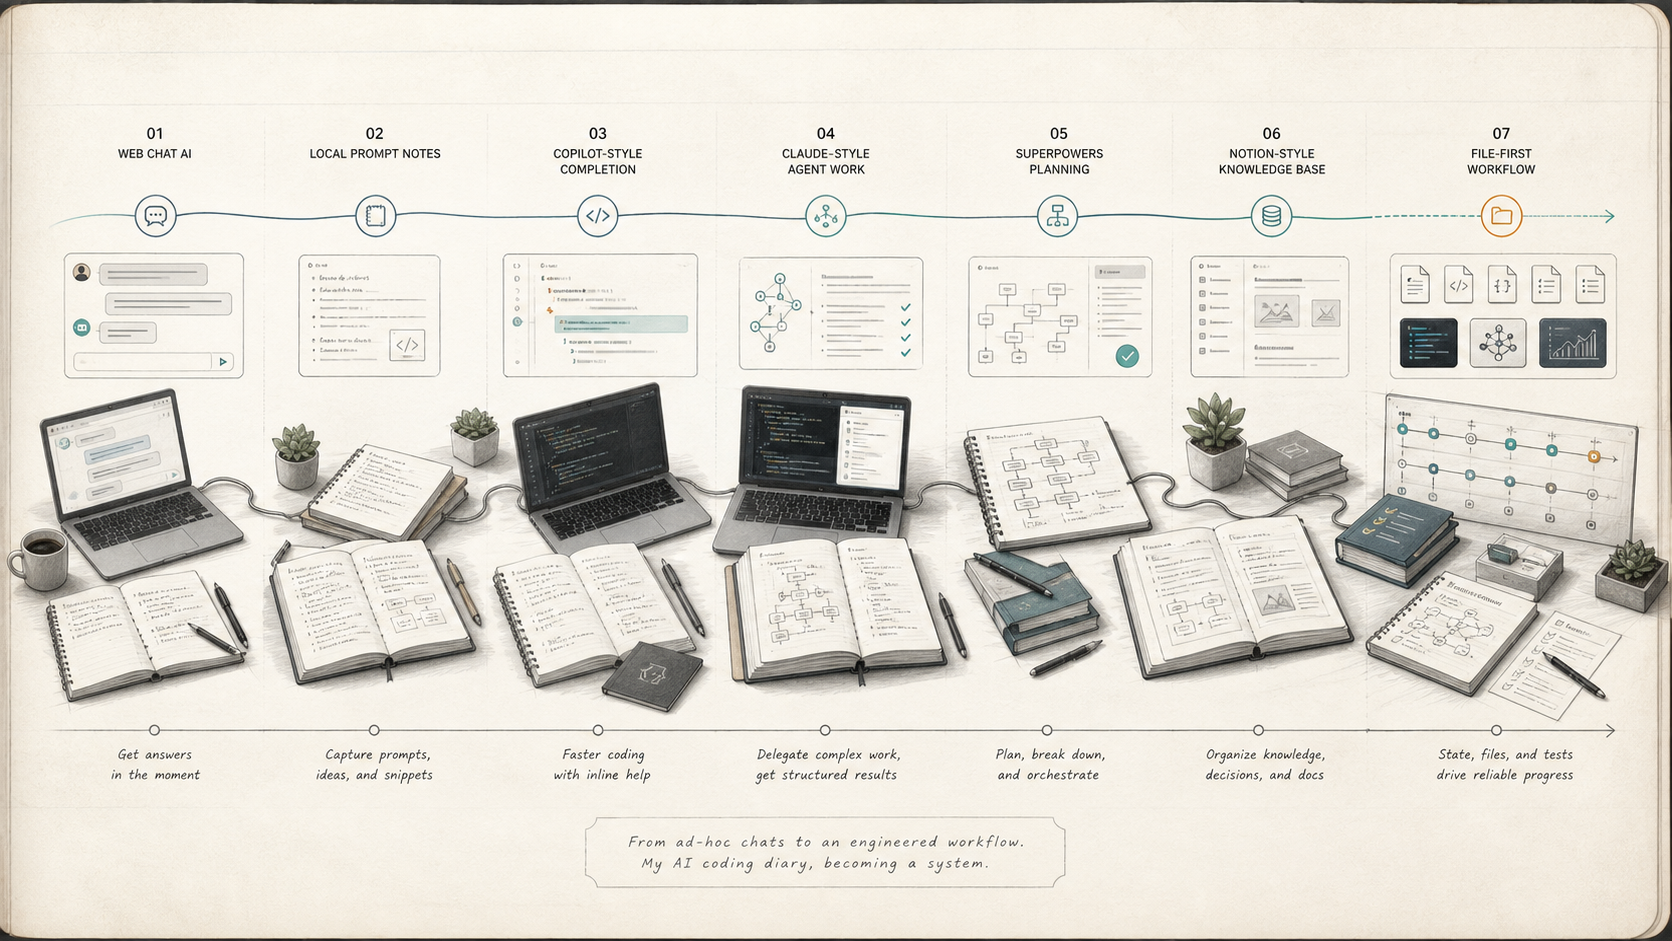
\includegraphics[width=\textwidth]{assets/gpt-image/tool-evolution-diary.png}
  \caption{从聊天式工具到结构化 Workflow 的演化脉络}
\end{figure}

\section{亲历的工具断裂：从 Hypo-LaTeX 到 Info 的小日记}

如果只把上面的迁移路线写成“工具 A 不够，所以换到工具 B”，这条历史会显得过于干净。真实情况要琐碎得多：每一次工具替换都不是一次漂亮的升级，而是在某个具体项目里被迫承认“这套办法再往下走会把人拖垮”。这些项目本身未必都是 Hypo-Workflow 的直接组成部分，但它们像一组连续实验，把同一个问题从不同角度暴露出来：AI 能在短时间里显得很聪明，却很难在长时间里稳定地承担工程责任。

Hypo-LaTeX 是一个很早的信号。当时作者主要依赖还没有 Skill / project memory 等能力的 Copilot。Copilot 对局部代码、模板续写和小范围修补很有效，但每当任务进入“维护项目秩序”这一层，它就开始显得吃力。例如让它补 \texttt{CHANGELOG}、遵守固定 Git 规范、按既有文档格式整理 release notes、不要乱改不相关文件，这些事情本来应该是项目规则的一部分，却需要作者在每次对话里重新粘贴一大段 prompt。那段时间最强烈的感受不是“模型不会”，而是“模型每次都像刚来这个项目”。它能在当前窗口里理解规则，却无法把规则变成下一次仍然可靠的行为。

更戏剧性的事情是，Copilot 连续被封 3 个账号。这个细节表面上像是账号使用问题，但在方法论上，它逼着作者承认一件事：不能把长期工作流压在单一服务、单一对话入口和单一交互习惯上。一个真正可依赖的工程流程，不能因为某个工具的账号、限流、策略变更或上下文丢失就整体停摆。也正是在这个阶段，“把规则写进外部文件而不是只写进聊天窗口”开始从一个偏好变成一个刚性需求。

\begin{example}{案例：Hypo-LaTeX 的 Prompt 搬运阶段}{case:hypo-latex}
\textbf{项目名：}Hypo-LaTeX。\\
\textbf{当时工具组合：}GitHub Copilot + 手工 prompt + 项目文档。\\
\textbf{做成了什么：}完成了 LaTeX 模板、变更说明、若干规范化文档和重复性维护任务。\\
\textbf{暴露了什么问题：}每次写 \texttt{CHANGELOG}、按 Git 规范提交、保持文档口径一致，都要把同一批规则重新粘贴给模型。Copilot 局部续写很强，但没有稳定的项目级行为记忆。\\
\textbf{促成的转向：}规则必须从 prompt 中移出来，沉淀为 Skill、template、release rule 或其他可复用资产；否则用户只是把“写代码”的负担换成了“重复喂 Prompt”的负担。
\end{example}

Bill 项目则把问题从“规则重复”推进到了“工程失控”。刚开始搭建时，Claude 的表现相当好：它能快速理解需求、生成界面、补齐一些显而易见的状态和交互。但当界面显示开始出问题时，体验迅速变味。作者会指出一个视觉或状态错误，模型给出一个看似合理的修补；修补之后另一个地方又坏掉；继续修，旧问题复发或者新问题出现。更麻烦的是，它并不会自然地把这些修补写成文档、决策记录或回归检查。于是几轮之后，表面上对话里一直在“解决问题”，实际上项目的可理解性越来越差。

这类失败很容易被误判为“模型能力不够”或者“prompt 没写清楚”。但从工程角度看，真正缺失的是全局变更边界、验证策略和文档同步机制。界面问题不是只能靠更聪明的下一次回答解决，它需要明确的验收方式：什么截图算通过，什么状态不允许退化，哪些组件不能被顺手重写，哪些设计约束必须留在文档里。没有这些外部结构，模型越勤快，项目反而越容易被局部修补搅乱。

\begin{example}{案例：Bill 的界面修补泥潭}{case:bill}
\textbf{项目名：}Bill。\\
\textbf{当时工具组合：}Claude + 临时对话式需求说明。\\
\textbf{做成了什么：}前期快速搭建了可运行界面和基础功能。\\
\textbf{暴露了什么问题：}后期 UI / 显示问题进入反复修补状态，模型经常“说一句话干半天”，最终结果却偏离真实需求；文档和回归证据没有同步沉淀，导致每次修复都像从头猜。\\
\textbf{促成的转向：}需要把“用户反馈”转化成明确验收证据，把视觉/交互问题纳入 Test Profile，而不是只靠下一轮自然语言解释。
\end{example}

Agent 项目让 Superpowers 的价值和边界同时变得清楚。Superpowers 前期确实非常好用：它让讨论先落盘，让模型在动手前写计划，让任务看起来不再只是松散聊天。这是作者第一次强烈感受到早期 Harness 的价值。它不是简单 prompt，而是把“先思考、再行动”的节奏外置出来，让模型不至于一上来就乱改文件。对于需求讨论、初始设计、功能分解，它的帮助很明显。

但 Agent 进入持续修 Bug 和加功能之后，Superpowers 的不足也开始暴露。它能在单次任务里形成局部计划，却不擅长维护跨任务的全局观。每次修改看起来都有理由，但理由往往只对当前问题负责；改一个地方，引入一串新的问题；再修新问题，又会冲淡旧设计。最终体验像是模型始终在“为了改而改”，而不是沿着一条可审计的工程轨道推进。这里并不是说 Superpowers 没用，恰恰相反，它的前期有效性证明了 Harness 方向是对的；但它作为早期 Harness 形态，还没有把状态、队列、评估、恢复和长期文档维护真正组合成系统。

\begin{example}{案例：Agent 与 Superpowers 的阶段性成功}{case:agent}
\textbf{项目名：}Agent。\\
\textbf{当时工具组合：}Claude + Superpowers。\\
\textbf{做成了什么：}前期讨论、计划落盘和功能起步效率明显提升。\\
\textbf{暴露了什么问题：}Superpowers 作为早期 Harness 能改善单次任务秩序，却缺少长期全局观；后期修 Bug 和加功能时，局部计划无法可靠约束跨模块影响，常常改一个引入一堆问题。\\
\textbf{促成的转向：}Harness 不能只是一套“动手前先计划”的提示，它必须拥有持久状态、feature queue、step 级检查、report 和 recovery 语义。
\end{example}

Research 和 Info 阶段则暴露出另一种疲劳：作者开始使用 Notion AI 管理文档、沉淀上下文，再把它生成的 prompt 复制给 Codex，让 Codex 执行、总结，再把结果搬回文档。这条路线在能力上比早期工具强很多，因为规划空间和执行空间终于被分开了；但人的角色也变得很尴尬。作者不再主要是“提出工程判断的人”，而更像是在 Notion AI 与 Codex 之间搬运 prompt、搬运结果、搬运上下文。这个阶段的结论非常刺眼：如果规划、状态、检索和执行不能通过协议连起来，那么再聪明的模型组合也会把用户夹在中间当胶水。

\begin{example}{案例：Research / Info 的搬运工阶段}{case:research-info}
\textbf{项目名：}Research / Info。\\
\textbf{当时工具组合：}Notion AI + 文档库 + Codex。\\
\textbf{做成了什么：}长期资料管理、语义检索、报告生成和局部实现能力都明显增强。\\
\textbf{暴露了什么问题：}规划在 Notion，执行在 Codex，状态同步靠作者复制粘贴；模型之间没有共享的生命周期协议，作者本质上变成 Prompt 搬运工。\\
\textbf{促成的转向：}Hypo-Workflow 必须让 plan、state、queue、progress、report、rules 和 execution evidence 都进入同一个文件优先协议，让人不再承担低价值搬运工作。
\end{example}

把这些片段连起来看，Hypo-Workflow 的问题定义就清楚了。它不是为了追赶某一个更强模型，也不是为了把某个工具包装得更好看，而是为了回答一个更朴素的问题：当用户已经知道 AI 可以帮忙写代码之后，如何让这种帮助在真实项目里持续、可恢复、可验证、可解释？从这个角度说，本报告后面的每个功能都不应被理解为“又加了一个模块”，而应被理解为“这个功能解决了怎样的问题”。其中一些能力来自用户反馈，例如对更清晰状态面板、Chat Mode、报告和 Slides 的要求；另一些能力则是作者主动设计出来的办法，例如 Feature Queue、Test Profiles、Progressive Discover 和 file-first recovery 语义。

\section{为什么“多写一点 Prompt”不是长期解法}

很多人第一次意识到 AI Coding 出问题时，会自然地想到一种补救方式：那就把 prompt 写得更详细一些，把规则列得更清楚一些，把上下文补得更全一些。但这种方案的根本问题在于，它把系统性问题转嫁给了人。

如果每次新会话开始，都要重新说明代码库结构、命名约定、交互方式、验收方法、文档要求、输出语言、禁止事项和上次做到哪里，那么所谓“AI 提效”其实只是把开发成本转移成了 prompt 维护成本。对一次性小任务，这种方法可能还凑合；对一个需要持续迭代、需要多人阅读、需要正式汇报的项目，它几乎一定会崩。

更糟的是，prompt 约束即使写得很长，也很难像文件协议一样稳定。它们会被截断、被覆盖、被后续局部细节稀释。换句话说，人类虽然能暂时把模型拉到正确轨道上，但如果轨道本身没有被工程化固化，模型最终仍然会回到“只对当前窗口负责”的局部优化状态。

\begin{important}{核心判断}{intro-judgement}
复杂 AI Coding 的主问题不是单次生成质量，而是长期状态管理、约束固化、验证闭环和中断恢复。
\end{important}

\section{本报告的目标与组织方式}

因此，这份报告试图回答三个问题：

\begin{enumerate}[leftmargin=2em]
  \item 从真实使用经验出发，AI Coding 到底受哪些结构性约束影响？
  \item 如果把这些约束当作工程问题来处理，应当得到怎样的系统设计？
  \item Hypo-Workflow 如何通过一组文件协议、Skills、rules、hooks、reports 和 adapters，把这些设计落地为可执行工作流？
\end{enumerate}

全文按以下逻辑展开：先说明 AI-assisted coding 的核心约束，再提出 Harness Engineering 这一设计视角；随后介绍 Hypo-Workflow 的文件优先协议、分层架构与恢复语义；之后用 V9 OpenCode Native Adapter 作为完整 case study；最后总结 C2 的关键扩展，包括 README 自动更新、Skill 质量治理、OpenCode 状态面板、Batch Planning、Chat Mode、Progressive Discover 与 Test Profiles，并给出面向实验室汇报的演示路线与未来工作。

\chapter{问题定义：AI-assisted coding 的核心约束}

\section{上下文窗口有限，全局观天然不稳定}

当任务涉及多个目录、多文件、历史设计决策和正式交付物时，模型面临的不是“会不会写某一段代码”，而是“能不能持续地维持全局约束”。上下文再长，也只能看到代码库的局部切片，而且会被临近话题覆盖。于是模型经常在局部正确、全局偏航的状态下持续推进。

\section{人工喂 Prompt 的成本会不断累积}

如果用户必须在每个会话里重新说明项目结构、风格要求、输出语言、测试方式和交付格式，那么这套系统本质上要求人来充当外部内存。随着项目时间拉长，这种做法的成本几乎线性增长。

\section{模型会“自己骗自己”}

这是一个很实际的工程问题。模型常常会生成\emph{语气上合理、结构上完整、但事实上不满足约束}的结果。例如：

\begin{itemize}[leftmargin=2em]
  \item 误判某个文件或目录已经存在；
  \item 误以为用户已经确认某种解释；
  \item 只跑单元测试就声称 WebApp 已验收通过；
  \item 在多轮迭代中逐渐偏离既有接口和架构边界。
\end{itemize}

一旦缺少外部检查点，模型就会不断在错误前提上继续推导。

\section{风格与行为难以固化}

很多工具能够“看起来像在记忆项目”，但这种记忆往往只是对当前窗口中显著模式的追随，而不是对长期行为协议的真正继承。没有 Skills、rules、templates、reports 这类外部资产，模型就很难长期稳定地输出同一种工程风格。

\section{中断、恢复和审计困难}

现实开发里，中断是常态。用户会切走去做别的事，会临时插入小修复，会在两个大任务之间聊一些补充问题。如果系统没有明确状态机，就无法回答三个基本问题：

\begin{enumerate}[leftmargin=2em]
  \item 现在做到哪里了？
  \item 下一步该从哪里继续？
  \item 如果最后结果出了问题，问题是在 Discover、Design、Implement 还是 Validation 阶段出现的？
\end{enumerate}

\section{从约束到系统需求}

这些问题不能只停留在体验抱怨层面，而必须转译成系统需求。表~\ref{tab:constraints} 给出了这种映射关系。

\begin{longtblr}[
  caption={AI Coding 约束到系统需求的映射},
  label={tab:constraints}
]{
  colspec={X[1,l]X[1.5,l]X[2,l]},
  row{1}={font=\bfseries},
  rowsep=3pt,
  hlines
}
\toprule
约束 & 直接后果 & Hypo-Workflow 对应机制 \\
\midrule
上下文窗口有限 & 只能稳定看见局部，容易丢全局 & \texttt{.pipeline/} 文件协议、compact 视图、reports、progress board \\
重复喂 prompt 成本高 & 用户每次都要重述规则和背景 & Skills、rules、templates、platform adapters \\
模型会自证正确 & 错误路径会越走越深 & evaluation、report、gates、required evidence、review steps \\
风格无法固化 & 命名、输出格式、交互方式漂移 & skill-quality、readme-spec、rules pack、command map \\
多轮迭代后偏航 & 先前设计意图难以保留 & Cycle / Feature / Milestone 分层与历史账本 \\
中断频繁 & 恢复成本高，下一步不清晰 & state.yaml、feature-queue.yaml、chat mode、patch 轨道 \\
\bottomrule
\end{longtblr}

\chapter{方法视角：Harness Engineering}

\section{什么是 Harness Engineering}

本项目采用的关键词是 \textbf{Harness Engineering}。这里的 harness 不是模型本体，而是围绕模型构建的一整套外部工程约束层：上下文、计划、状态、规则、评估、恢复与协作协议都被显式写入文件和工具中，让模型始终运行在一条可审计、可恢复、可迭代的工程轨道上。

\section{四个核心原则}

这一定义可以被拆成四个直接的设计原则：

\begin{enumerate}[leftmargin=2em]
  \item \textbf{执行闭环}：Plan、Execute、Review、Report、Evaluate、Recover 组成循环，而不是彼此断裂的聊天片段。
  \item \textbf{分层建模}：Project、Cycle、Feature、Milestone、Patch、Step、Report 各自承担不同粒度的决策。
  \item \textbf{行为固化}：Skills、rules、hooks、templates、adapters 承担“反复重复的约束”。
  \item \textbf{自动维护}：README、PROGRESS、reports、queue、metrics、release checks 由 workflow 自动刷新。
\end{enumerate}

\begin{figure}[H]
  \centering
  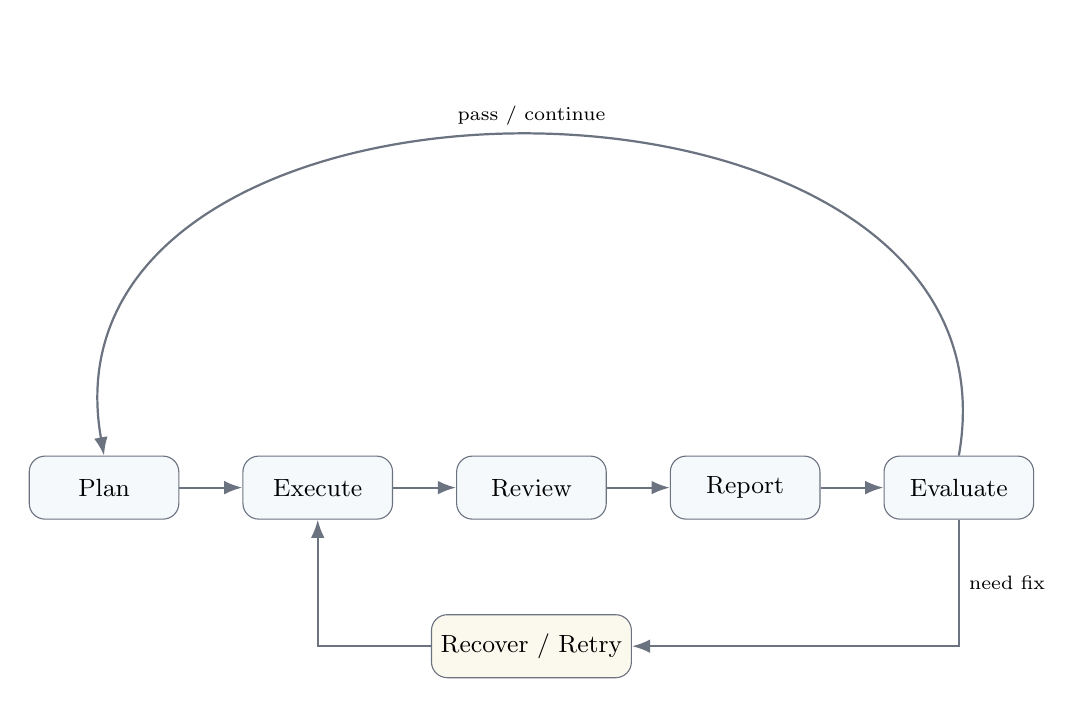
\begin{tikzpicture}[
  node distance=10mm and 8mm,
  box/.style={draw=HWGray, rounded corners=2mm, fill=HWBlue!8, minimum width=19mm, minimum height=8mm, align=center, font=\small},
  arrow/.style={-Latex, thick, draw=HWGray}
]
\node[box] (plan) {Plan};
\node[box, right=of plan] (execute) {Execute};
\node[box, right=of execute] (review) {Review};
\node[box, right=of review] (report) {Report};
\node[box, right=of report] (evaluate) {Evaluate};
\node[box, below=12mm of review, fill=HWGold!18] (recover) {Recover / Retry};
\draw[arrow] (plan) -- (execute);
\draw[arrow] (execute) -- (review);
\draw[arrow] (review) -- (report);
\draw[arrow] (report) -- (evaluate);
\draw[arrow] (evaluate.south) |- node[pos=0.25, right, font=\scriptsize]{need fix} (recover.east);
\draw[arrow] (recover.west) -| (execute.south);
\draw[arrow] (evaluate.north) to[out=80, in=100, looseness=1.3] node[above, font=\scriptsize]{pass / continue} (plan.north);
\end{tikzpicture}

  \caption{Hypo-Workflow 的执行闭环}
\end{figure}

\section{为什么这不是“再造一个 Runner”}

Hypo-Workflow 的关键判断之一是：它不需要自己再造一套执行器。真正执行代码生成与实现工作的，仍然是宿主 Agent，例如 Codex、Claude Code 或 OpenCode。Hypo-Workflow 提供的是围绕这些 Agent 的约束协议和状态系统，而不是替代它们本身。

这一区分很重要。因为一旦 workflow 既想控制状态、又想接管执行、又想提供平台特定 UI，很容易陷入重复发明底层能力的陷阱。Hypo-Workflow 选择的路线是：\emph{统一 contract，多平台 adapter，宿主负责实际推理与执行。}

\chapter{Hypo-Workflow 总体架构}

\section{文件优先协议}

Hypo-Workflow 的核心判断是：对长流程 AI work 来说，\textbf{文件比聊天窗口更适合作为状态容器}。因此项目把 \texttt{.pipeline/} 视为事实来源，而不是把长期状态埋进对话历史里。

\begin{figure}[H]
  \centering
  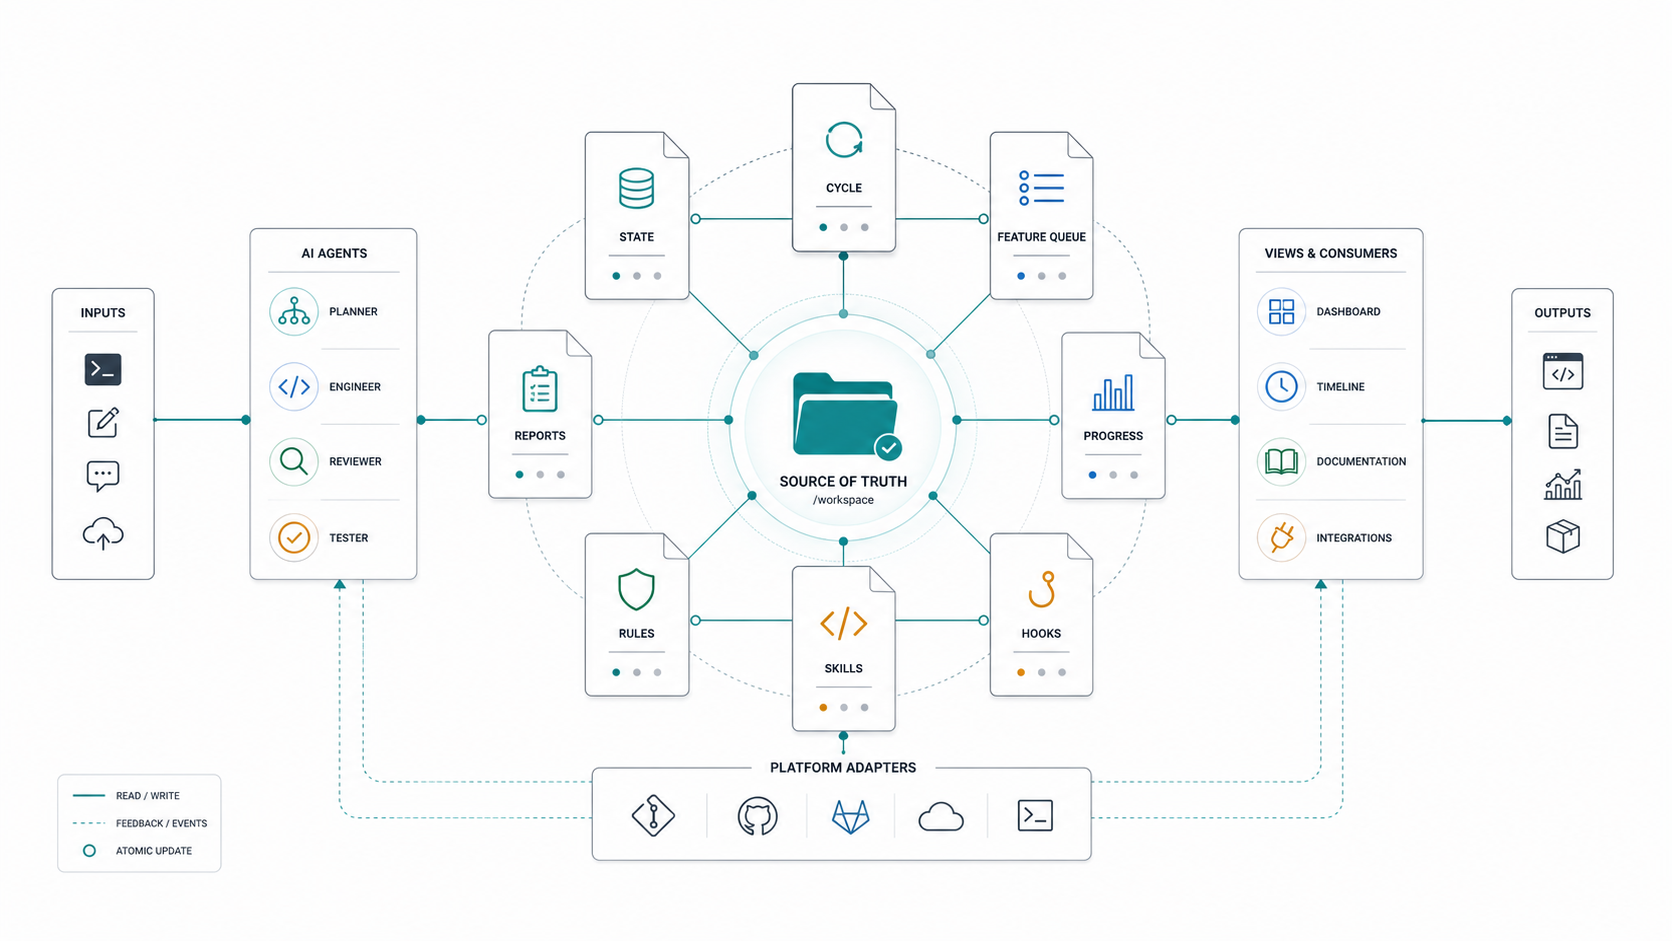
\includegraphics[width=\textwidth]{assets/gpt-image/file-first-architecture.png}
  \caption{File-first architecture 概念图}
\end{figure}

\begin{figure}[H]
  \centering
  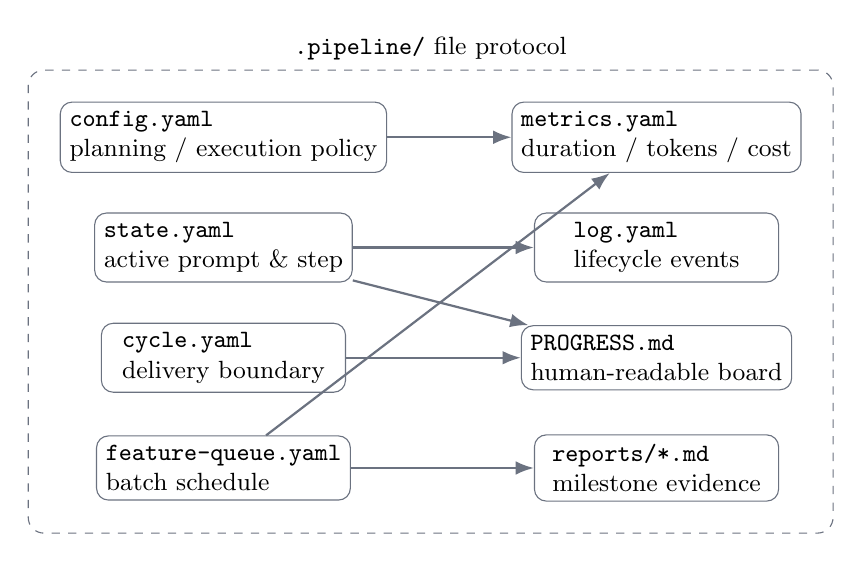
\begin{tikzpicture}[
  file/.style={draw=HWGray, rounded corners=1.5mm, fill=white, minimum width=31mm, minimum height=8mm, align=left, font=\small},
  group/.style={draw=HWGray, rounded corners=2mm, dashed, inner sep=4mm},
  arrow/.style={-Latex, thick, draw=HWGray}
]
\node[file] (config) at (0,2.2) {\texttt{config.yaml}\\planning / execution policy};
\node[file] (state) at (0,0.8) {\texttt{state.yaml}\\active prompt \& step};
\node[file] (cycle) at (0,-0.6) {\texttt{cycle.yaml}\\delivery boundary};
\node[file] (queue) at (0,-2.0) {\texttt{feature-queue.yaml}\\batch schedule};
\node[file] (metrics) at (5.5,2.2) {\texttt{metrics.yaml}\\duration / tokens / cost};
\node[file] (log) at (5.5,0.8) {\texttt{log.yaml}\\lifecycle events};
\node[file] (progress) at (5.5,-0.6) {\texttt{PROGRESS.md}\\human-readable board};
\node[file] (reports) at (5.5,-2.0) {\texttt{reports/*.md}\\milestone evidence};

\node[group, fit=(config)(state)(cycle)(queue)(metrics)(log)(progress)(reports), label=above:{\small \texttt{.pipeline/} file protocol}] {};

\draw[arrow] (config.east) -- (metrics.west);
\draw[arrow] (state.east) -- (log.west);
\draw[arrow] (cycle.east) -- (progress.west);
\draw[arrow] (queue.east) -- (reports.west);
\draw[arrow] (state) -- (progress);
\draw[arrow] (queue) -- (metrics);
\end{tikzpicture}

  \caption{\texttt{.pipeline/} 文件协议}
\end{figure}

\section{关键文件职责}

\begin{longtblr}[
  caption={关键文件职责},
  label={tab:files}
]{
  colspec={X[1,l]X[3.5,l]},
  row{1}={font=\bfseries},
  rowsep=3pt,
  hlines
}
\toprule
文件 & 作用 \\
\midrule
\texttt{state.yaml} & 当前执行到哪个 prompt、哪个 step、最近质量评分、历史完成项和可恢复状态。\\
\texttt{cycle.yaml} & 当前交付 Cycle 的边界、摘要、经验教训和归档语义。\\
\texttt{feature-queue.yaml} & Batch Plan 的 Feature 级调度层、gate 与状态摘要。\\
\texttt{metrics.yaml} & duration、tokens、cost 等可选遥测数据。\\
\texttt{log.yaml} & 生命周期事件账本。\\
\texttt{PROGRESS.md} & 面向人类阅读的进度板。\\
\texttt{reports/*.md} & 每个 Milestone 的交付说明、测试结论和评价。\\
\bottomrule
\end{longtblr}

\section{项目资产规模与观测对象}

截至本报告编写时，仓库已经形成一组足够说明问题规模的工程资产：

\begin{itemize}[leftmargin=2em]
  \item 用户可见命令 31 个，另有 1 个内部 watchdog Skill；
  \item 本地 Skill 文件 31 份；
  \item \texttt{core/src} 共 14 个实现文件；
  \item \texttt{references/} 共 28 份规范或对照文档；
  \item C2 共 19 个 Milestone prompt；
  \item 当前核心测试达到 70/70 通过；
  \item Git 跟踪文件总数为 495。
\end{itemize}

这些数字的意义不在于“资产越多越好”，而在于它们表明 Hypo-Workflow 已经不是单一 prompt 工具，而是一个包含命令面、状态协议、平台适配、规则系统、文档与回归测试的完整工程体。

\section{层级关系}

\begin{figure}[H]
  \centering
  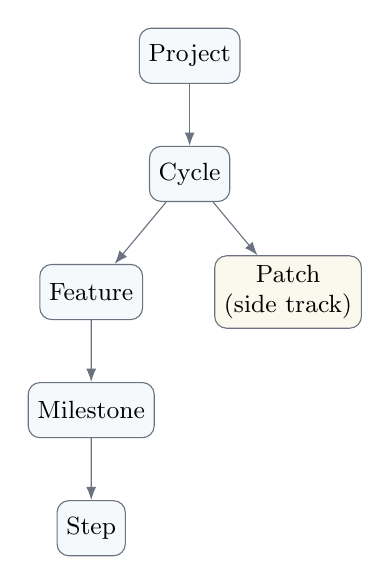
\begin{tikzpicture}[
  level 1/.style={sibling distance=40mm},
  level 2/.style={sibling distance=25mm},
  level 3/.style={sibling distance=18mm},
  every node/.style={draw=HWGray, rounded corners=1.5mm, fill=HWBlue!8, font=\small, align=center, minimum height=7mm},
  edge from parent/.style={draw=HWGray, -Latex}
]
\node {Project}
  child { node {Cycle}
    child { node {Feature} 
      child { node {Milestone} 
        child { node {Step} }
      }
    }
    child { node[fill=HWGold!18] {Patch\\(side track)} }
  };
\end{tikzpicture}

  \caption{Project / Cycle / Feature / Milestone / Step 与 Patch 的关系}
\end{figure}

其中：

\begin{itemize}[leftmargin=2em]
  \item \textbf{Cycle} 是一次交付边界，负责归档、生命周期和阶段性目标；
  \item \textbf{Feature} 是 batch plan 中的需求调度单元；
  \item \textbf{Milestone} 是可执行 prompt/report 单元；
  \item \textbf{Step} 是 TDD 或 implement-only 序列中的执行阶段；
  \item \textbf{Patch} 是轻量修复旁路，不强制并入主 Milestone 流。
\end{itemize}

\section{失败恢复与状态推进}

长流程系统如果只定义成功路径，几乎一定会在真实使用中失效。Hypo-Workflow 因此把若干非成功路径也纳入正式协议：

\begin{itemize}[leftmargin=2em]
  \item \textbf{gate: confirm}：在特定 Feature 前暂停，让用户确认是否继续；
  \item \textbf{skip / defer}：当需求阻塞或收益不足时，允许显式跳过；
  \item \textbf{Patch}：小修复不强行回灌到主 Milestone；
  \item \textbf{Chat Mode}：轻量追问和小修改进入追加对话轨道；
  \item \textbf{Stop / Resume}：会话可安全暂停，并由状态文件恢复。
\end{itemize}

\chapter{V9 OpenCode Native Adapter Case Study}

\section{为什么选 V9 作为案例}

V9 是一个非常合适的 case study，因为它不是概念层的讨论，而是一轮完整的、可归档的工程交付：在 C1 中共完成 10 个里程碑，最终形成 OpenCode native adapter、global CLI、command mapping、plugin scaffold、TUI 扩展基础、文档和 release 准备。归档摘要保存在 \texttt{.pipeline/archives/C1-v9-opencode-native-adapter/summary.md}。

\section{核心问题}

OpenCode 适配的技术问题不是“能不能生成一份命令表”，而是如何在不把 Hypo-Workflow 变成 runner 的前提下，提供原生 slash command、agent roles、event policy、file guard 与状态展示。

\section{架构原则}

\texttt{references/v9-architecture.md} 中明确了几个原则：

\begin{itemize}[leftmargin=2em]
  \item 一套 workflow contract，多平台 adapter；
  \item OpenCode 原生能力优先，不重复发明执行机制；
  \item deterministic generation 进入 \texttt{core/}；
  \item 实际推理与实现仍由宿主 Agent 完成；
  \item \texttt{.pipeline/} 保持跨平台 source of truth。
\end{itemize}

\begin{figure}[H]
  \centering
  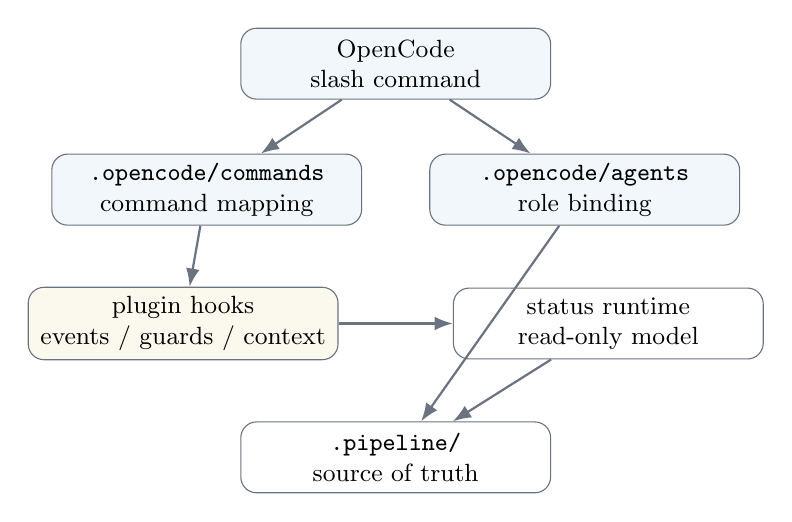
\begin{tikzpicture}[
  box/.style={draw=HWGray, rounded corners=2mm, minimum width=31mm, minimum height=9mm, text width=30mm, align=center, font=\small},
  wide/.style={box, minimum width=39mm, text width=37mm},
  arrow/.style={-Latex, thick, draw=HWGray}
]
\node[wide, fill=HWBlue!10] (user) at (0,2.4) {OpenCode\\slash command};
\node[wide, fill=HWBlue!10] (cmd) at (-2.4,0.8) {\texttt{.opencode/commands}\\command mapping};
\node[wide, fill=HWBlue!10] (agent) at (2.4,0.8) {\texttt{.opencode/agents}\\role binding};
\node[wide, fill=HWGold!18] (plugin) at (-2.7,-0.9) {plugin hooks\\events / guards / context};
\node[wide, fill=white] (runtime) at (2.7,-0.9) {status runtime\\read-only model};
\node[wide, fill=white] (pipeline) at (0,-2.6) {\texttt{.pipeline/}\\source of truth};

\draw[arrow] (user) -- (cmd);
\draw[arrow] (user) -- (agent);
\draw[arrow] (cmd) -- (plugin);
\draw[arrow] (plugin) -- (runtime);
\draw[arrow] (runtime) -- (pipeline);
\draw[arrow] (agent) -- (pipeline);
\end{tikzpicture}

  \caption{OpenCode Native Adapter 结构}
\end{figure}

\begin{figure}[H]
  \centering
  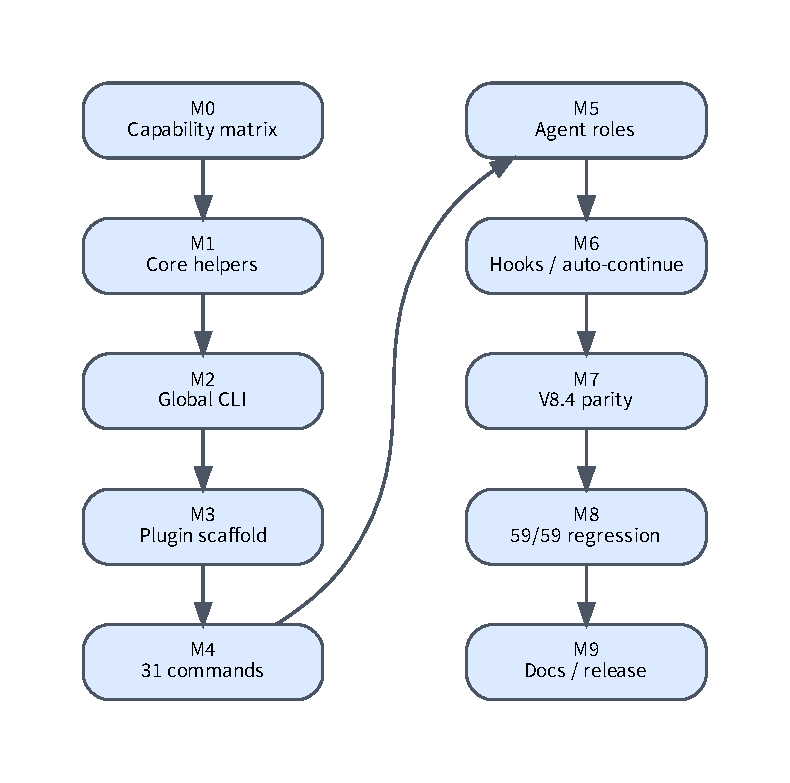
\includegraphics[width=\textwidth]{figures/v9-timeline.pdf}
  \caption{V9 OpenCode Native Adapter 时间线}
\end{figure}

\section{几个关键工程判断}

\begin{enumerate}[leftmargin=2em]
  \item \texttt{core/} 只承载 deterministic helper，不承担 runner 语义；
  \item 命令映射必须可测试，而不是文档里的一张静态表；
  \item plugin 与 runtime helper 分离，避免被 OpenCode 错误扫描；
  \item regression suite 不是装饰品，而是交付证据的一部分。
\end{enumerate}

\section{为什么 V9 说明这套方法有效}

V9 的价值不只是“支持了 OpenCode”，而是它把一组原本容易散落在聊天记录中的设计约束，落到了可验证资产中：capability matrix、platform adapter、Ask/todowrite 纪律、file guard、bootstrap artifact、文档和 release metadata 都进入了工程系统。

\chapter{功能如何按问题长出来}

\section{从“功能清单”改成“问题账本”}

如果把 C2 写成一串功能名，它会显得很像普通迭代记录：README 自动更新、Skill 质量治理、OpenCode 面板、Batch Planning、Chat Mode、Progressive Discover、Test Profiles、Showcase。这样的写法虽然准确，却没有解释为什么这些功能必须出现。更贴近真实开发过程的说法是：每个功能都是某种反复出现的问题留下来的疤痕，然后被转译成协议、测试或交互面。

因此，本章不刻意区分“这是 C2 的第几个 Milestone”，而是沿着问题演化来写：当项目资产变多，README 会过时；当 Skill 变多，行为约束会漂移；当 Feature 变多，单一 Milestone 序列不够表达计划；当用户不想反复查状态，就需要只读观测面；当 Cycle 结束后仍有小讨论，就需要 Chat Mode；当需求还没讲清楚时，就需要 Progressive Discover；当不同任务的验收标准不同，就需要 Test Profiles。这些功能共同回答一个问题：Hypo-Workflow 如何让 AI work 不再靠人临场维持秩序。

\section{README 自动更新：解决“入口文档总是慢半拍”的问题}

README 是一个项目最常被阅读、也最容易过时的文件。对一个普通库来说，README 过时已经很麻烦；对 Hypo-Workflow 这种命令、Skill、adapter、rules、profiles 都在演化的项目来说，README 一旦过时，就会直接误导用户如何启动、如何恢复、如何选择命令。C2 之前，README 的维护很大程度依赖人工记忆：功能改了、命令数量变了、平台支持变了，需要作者自己想起来同步。

这正是 Hypo-LaTeX 阶段暴露过的问题的工程化版本：不要让人每次都充当文档同步器。于是 C2 把 README 维护拆成两层。第一层是 \texttt{templates/readme-spec.md}，它定义哪些内容属于动态区块、哪些数据源可以被机器读取、哪些文字仍然应该由人维护。第二层是 release 路径中的 \texttt{update\_readme} 与 \texttt{readme-freshness}，前者负责刷新，后者负责阻止明显过时的发布。

这个设计的重点不是自动生成整份 README。完全自动生成反而会破坏文档的叙事和可读性。更稳妥的边界是：人负责解释项目，机器负责刷新那些本来就应该由事实源驱动的部分，例如版本号、命令数量、Skill 清单、测试结果和平台矩阵。这样一来，README 不再是 release 之后“想起来再补”的文件，而是 release gate 的一部分。

\section{Skill 体系整理：解决“行为约束越多越难管”的问题}

Skill 的价值在于把反复出现的行为要求从 prompt 中拿出来，让模型在合适场景下自动加载更专业的操作方式。但 Skill 一多，新的风险就出现了：frontmatter 不一致、触发描述过宽或过窄、命名漂移、引用路径过时、平台说明冲突、输出语言规则不一致。也就是说，Skill 本来是为了解决 prompt 重复，结果它自己也会变成需要治理的资产。

C2 的做法是把 Skill 当作一类正式工程对象，而不是一堆“看起来有用的 Markdown”。\texttt{references/skill-spec.md} 定义 Skill 应该包含哪些元信息、如何描述触发条件、如何引用本地资源、如何避免互相覆盖；\texttt{skill-quality} 规则则把这些约束纳入检查面。这个功能解决的问题很具体：当未来新增或修改 Skill 时，作者不需要凭感觉判断“这样写差不多吧”，而可以让规则检查暴露明显的不一致。

这里也能看到 Harness Engineering 的第二条主轴：行为固化不是一次性动作，而是需要维护的资产系统。Copilot 时代的重复 prompt 被抽成 Skill；Skill 继续增长后，又需要 spec 和 quality rule 来维护它。Hypo-Workflow 的设计并不是把复杂性消灭掉，而是把复杂性放到更可检查的位置。

\section{OpenCode 状态面板：解决“状态事实源看得见”的问题}

C2 的 M08/M09 为 OpenCode 增加了只读状态面板。其本质，是把 \texttt{.pipeline/} 的状态投影到 TUI，而不是另造一个 UI 状态系统。这样用户不必反复手动运行 \texttt{/hw:status}，就能看到当前 Cycle、Feature、Milestone、最近事件以及 duration / token / cost 摘要。

\begin{figure}[H]
  \centering
  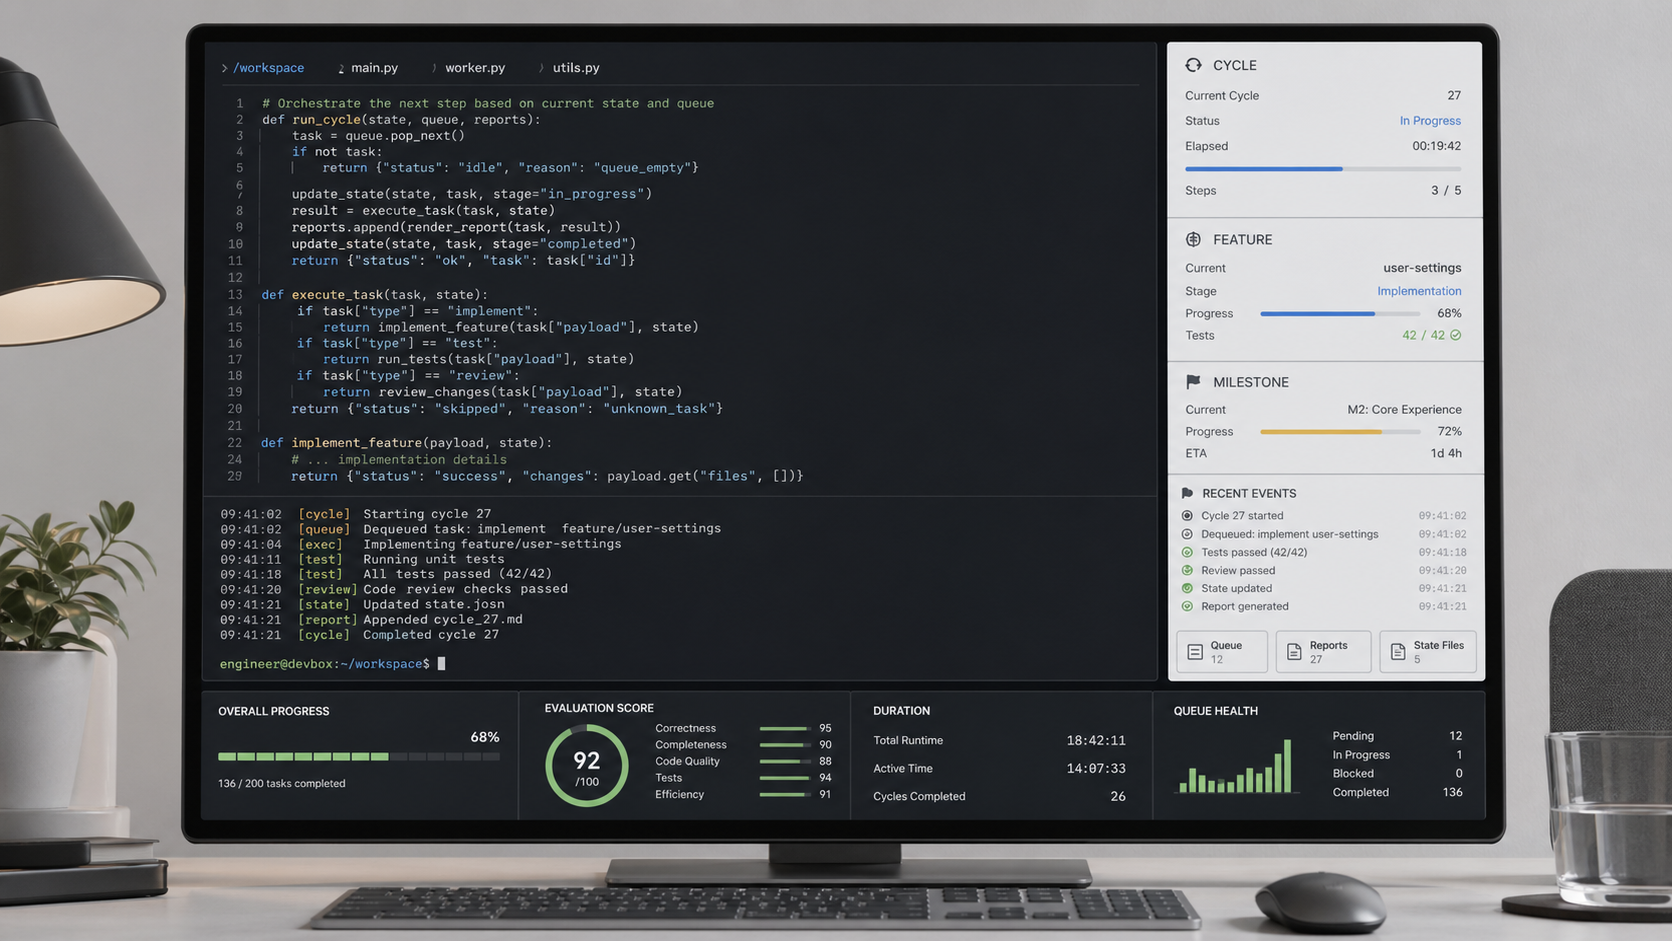
\includegraphics[width=\textwidth]{assets/opencode-observability.png}
  \caption{OpenCode 侧边栏与底部状态面板的展示意图}
\end{figure}

只读这两个字很重要。很多 workflow UI 容易犯的错误，是在界面层重新维护一份状态，然后让它和底层文件逐渐不一致。Hypo-Workflow 选择反过来：\texttt{state.yaml}、\texttt{feature-queue.yaml}、\texttt{log.yaml}、\texttt{PROGRESS.md} 仍然是事实源，OpenCode 面板只是读它们、整理它们、把它们放到用户工作时自然能看到的地方。这样既保留了 file-first 的可审计性，也降低了用户频繁查询状态的摩擦。

\section{Batch Planning：解决“多功能计划没有调度层”的问题}

早期 Plan 流更适合单一 Feature：用户提出一个目标，Discover 澄清，Decompose 拆 Milestone，Generate 产 prompt，Confirm 后执行。但 C2 的真实需求明显更复杂：README、Skill、OpenCode UI、Batch、Report、Chat、Discover、Profiles 这些能力并不是一个线性小任务，而是一组有依赖、有优先级、有 gate 的 Feature。如果每个 Feature 都重新跑一次完整计划，用户会被流程本身拖慢；如果直接把所有东西塞进一个大 prompt，执行又会失控。

Batch Plan 引入了 \texttt{Feature Queue} 这一层。它允许用户在一次 Discover 中规划多个 Feature，并选择 upfront 或 just-in-time decomposition，然后由系统按顺序 auto-chain 推进。Feature Queue 的作用不是替代 Milestone，而是在 Cycle 和 Milestone 中间补上“用户需求单元”这一层：Feature 记录真正要解决的问题，Milestone 记录为了解决它而拆出的可执行步骤。

这也解释了为什么 Batch Plan 不是普通任务列表。普通 TODO 只能告诉系统“还有什么没做”，而 Feature Queue 还要表达 gate、decompose mode、failure policy、priority、metric summary 和 prompt path。它让系统在推进时能回答：下一个 Feature 是什么？是否需要用户确认？是 upfront 分解还是 JIT 分解？失败后是停止、跳过还是延期？这些信息一旦进入文件协议，Agent 就不必在每次继续时重新猜测调度策略。

\section{Chat Mode：解决“轻量后续讨论无法归档”的问题}

\texttt{/hw:chat} 处理的是一个很真实的场景：用户在 Cycle 完成后，常有轻量追问、小修改和小讨论。这些需求不足以开启新 Patch 或新 Cycle，但如果完全放在随意对话里，workflow 上下文又会迅速丢失。Chat Mode 通过 \texttt{chat:} 状态和 \texttt{chat\_entry} 账本，把这类互动纳入可恢复轨道。

这个功能很像前面 Research / Info 阶段的反面。当时作者在 Notion AI 和 Codex 之间手工搬运上下文，是因为讨论空间和执行空间没有协议连接。Chat Mode 不试图把所有闲聊都升级成正式 Milestone，而是给“还没有到 Patch 级别、但又不能完全丢掉”的信息一个轻量容器。它可以记录用户补充了什么、系统如何回应、是否应该升级为 Patch 或 Plan Extend。这样一来，小讨论不再是会话里的烟雾，而是可以在后续恢复时被看见的上下文。

\section{Progressive Discover：解决“还没问清就开始计划”的问题}

Progressive Discover 的目标不是“多问几轮”，而是控制 Discover 的顺序。先问 task category、desired effect、verification method，再进入 assumption statement、ambiguity resolution、tradeoff review 和 validation criteria。

\begin{figure}[H]
  \centering
  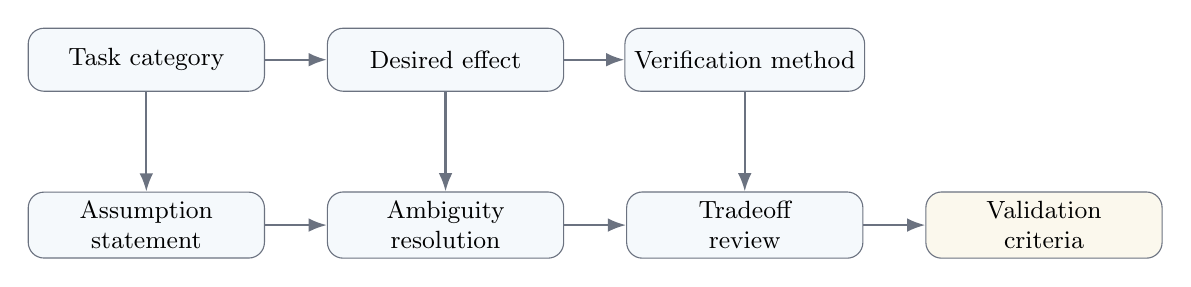
\begin{tikzpicture}[
  stage/.style={draw=HWGray, rounded corners=2mm, fill=HWBlue!8, minimum width=30mm, minimum height=8mm, align=center, font=\small},
  arrow/.style={-Latex, thick, draw=HWGray}
]
\node[stage] (q1) at (0,2.1) {Task category};
\node[stage] (q2) at (3.8,2.1) {Desired effect};
\node[stage] (q3) at (7.6,2.1) {Verification method};
\node[stage] (s1) at (0,0) {Assumption\\statement};
\node[stage] (s2) at (3.8,0) {Ambiguity\\resolution};
\node[stage] (s3) at (7.6,0) {Tradeoff\\review};
\node[stage, fill=HWGold!18] (s4) at (11.4,0) {Validation\\criteria};
\draw[arrow] (q1) -- (q2);
\draw[arrow] (q2) -- (q3);
\draw[arrow] (q1.south) -- (s1.north);
\draw[arrow] (q2.south) -- (s2.north);
\draw[arrow] (q3.south) -- (s3.north);
\draw[arrow] (s1) -- (s2);
\draw[arrow] (s2) -- (s3);
\draw[arrow] (s3) -- (s4);
\end{tikzpicture}

  \caption{Progressive Discover 结构}
\end{figure}

这个顺序来自一个简单观察：很多失败并不是发生在实现阶段，而是发生在最开始的问题定义阶段。模型很容易在目标还模糊时就急着给方案，用户也很容易被一个看起来完整的计划带走。Progressive Discover 要求先把大问题问出来：这是 WebApp、agent-service、research 还是文档工作？用户真正想看到的效果是什么？最终应该怎样验证？这些问题回答不清楚，后面的 Milestone 拆得再漂亮也可能是错的。

\section{Test Profiles：解决“所有任务都用同一种通过定义”的问题}

Test Profile 是 C2 最关键的新概念之一。它明确区分：

\begin{itemize}[leftmargin=2em]
  \item \textbf{preset}：决定 step sequence，例如 tdd / implement-only；
  \item \textbf{profile}：决定 validation policy，例如 webapp / agent-service / research。
\end{itemize}

\begin{figure}[H]
  \centering
  \begin{tblr}{
    colspec={X[1,l]X[2,l]X[2.5,l]X[2,l]},
    row{1}={bg=HWBlue!10,font=\bfseries},
    rowsep=3pt,
    hlines
  }
    \toprule
    Profile & Discover focus & Required evidence & Forbidden shortcut \\
    \midrule
    webapp & browser path / visual effect & E2E + browser interaction + screenshot & unit test only \\
    agent-service & CLI shape / shared core & CLI plan + shared core + real CLI run & split core logic \\
    research & baseline / direction / script & before + after + delta + script execution & diff-only acceptance \\
    \bottomrule
  \end{tblr}
  \caption{Test Profile 矩阵}
\end{figure}

这一设计的核心判断是：\emph{不同任务类型的“通过”定义并不相同。} WebApp 需要 E2E 和可视证据，Agent / Service 需要真实 CLI 调用与 shared core，Research 需要 baseline / script / delta，而不是只看 diff。

这项能力直接回应了 Bill 和 Agent 阶段的失败。Bill 的 UI 问题不能只靠单元测试说通过，它需要截图、交互路径、移动端/桌面端视口检查和视觉不重叠证据。Agent-service 类任务不能只看某个 helper 函数输出正确，还要看真实 CLI 或服务路径是否能跑通。Research 类任务也不能只看文本是否生成，而要比较 baseline、脚本输出和 delta。Test Profile 把这些差异提前放到 Plan 阶段，迫使系统在动手前定义“什么才算完成”。

\section{Feature / Cycle / Milestone / Patch 关系澄清}

这几个概念在很多 AI workflow 中容易混用，因此这里明确给出定义：

\begin{itemize}[leftmargin=2em]
  \item \textbf{Cycle}：一次阶段性交付；
  \item \textbf{Feature}：用户真正想解决的问题单元；
  \item \textbf{Milestone}：为交付某个 Feature 而拆出的可执行 prompt / report 单元；
  \item \textbf{Patch}：独立于主序列的小修复旁路。
\end{itemize}

\chapter{完整工作流切片与演示路径}

\section{一个典型切片}

假设用户希望连续完成多个功能，其中既包括 WebApp UI，也包括一个研究脚本优化。Hypo-Workflow 的处理方式并不是直接进入实现，而是先确定类别、效果和验证方式：

\begin{enumerate}[leftmargin=2em]
  \item 这个任务属于什么类别：webapp、agent-service、research，还是一般代码维护？
  \item 希望达到怎样的效果：用户可见行为、性能指标、交互流程还是架构边界？
  \item 准备如何验证：浏览器 E2E、CLI 场景、benchmark 脚本，还是别的方式？
\end{enumerate}

如果用户选择 \texttt{/hw:plan --batch}，Discover 会一次性覆盖多个 Feature，并输出 \texttt{feature-queue.yaml}。随后系统再根据 queue 顺序和 gate 策略，决定何时进入 Milestone 分解和执行。

\section{Demo Route}

最终演示建议按下面路径组织：

\begin{enumerate}[leftmargin=2em]
  \item 从 \texttt{README.md} 与 \texttt{.pipeline/PROGRESS.md} 开始，说明 file-first workflow；
  \item 用 \texttt{/hw:plan} 或 \texttt{/hw:plan --batch} 展示 Progressive Discover 的入口问题；
  \item 展示 \texttt{feature-queue.yaml}，解释 Feature 层调度；
  \item 引入 Test Profiles，说明“怎么验证”在 Plan 阶段就被定义；
  \item 展示 OpenCode 状态面板文件与运行路径；
  \item 展示 \texttt{/hw:chat} 如何承接轻量后续讨论；
  \item 展示 \texttt{/hw:release} 如何做 README 更新与 release gate；
  \item 最后以 tests、reports 和 PDF 产物证明闭环完成。
\end{enumerate}

\section{验证矩阵}

\begin{longtblr}[
  caption={C2 Validation Matrix},
  label={tab:validation}
]{
  colspec={X[1.2,l]X[2.2,l]X[2.4,l]X[2,l]},
  row{1}={bg=HWBlue!10,font=\bfseries},
  rowsep=3pt,
  hlines
}
\toprule
能力 & 关键证据 & 自动化验证 & 备注 \\
\midrule
README 自动更新 & {\small\ttfamily templates/readme-spec.md}、README managed blocks & {\small\ttfamily core/test/readme-update.test.js}；{\small\ttfamily checkReadmeFreshness()} & 发版路径要求通过 freshness gate \\
Skill 质量治理 & {\small\ttfamily references/skill-spec.md}、Skill frontmatter/headings & {\small\ttfamily core/test/skill-quality.test.js}；{\small\ttfamily checkSkillQuality()} & 当前仓库结果为 0 issues / 31 Skill 文件 \\
OpenCode 状态面板 & status runtime、sidebar/footer plugin & {\small\ttfamily core/test/opencode-status.test.js}；{\small\ttfamily core/test/opencode-panels.test.js} & 只读投影，不直接改 workflow 状态 \\
Batch Planning & Feature Queue、Markdown artifact、Mermaid/TikZ 图 & {\small\ttfamily core/test/batch-plan.test.js}；{\small\ttfamily core/test/feature-queue-ops.test.js} & 普通单功能 {\small\ttfamily /hw:plan} 行为保持不变 \\
Chat Mode & {\small\ttfamily chat:} state、{\small\ttfamily chat\_entry}、Stop/SessionStart Hook & {\small\ttfamily core/test/chat-*.test.js} & 轻量讨论与主 Milestone 流分离 \\
Progressive Discover & category/effect/verification big questions & {\small\ttfamily core/test/progressive-discover.test.js} & 支持 optional {\small\ttfamily @karpathy/guidelines} \\
Test Profiles & webapp / agent-service / research evidence contracts & {\small\ttfamily core/test/test-profile.test.js} & 验证策略前置到 Plan 阶段 \\
项目展示交付 & report.tex、slides.tex、PDF、demo script & XeLaTeX build、全量回归、diff check & 最终产出可直接用于实验室汇报 \\
\bottomrule
\end{longtblr}

\chapter{讨论：与其他工具的关系}

\section{工具对比}

\begin{longtblr}[
  caption={AI 工具能力对比},
  label={tab:compare}
]{
  colspec={X[1.3,l]X[l]X[l]X[l]X[l]X[l]X[l]X[l]},
  row{1}={bg=HWBlue!10,font=\bfseries,font=\small},
  row{2-Z}={font=\small},
  rowsep=2pt,
  hlines
}
\toprule
工具 & Repo & Plan & Context & Recover & Style & Auto & Valid. \\
\midrule
Web GPT / Gemini & 弱 & 弱 & 弱 & 弱 & 弱 & 无 & 弱 \\
Cherry Studio + DeepSeek & 弱 & 弱 & 弱 & 弱 & 弱 & 无 & 弱 \\
GitHub Copilot & 中 & 弱 & 弱 & 弱 & 弱 & 无 & 弱 \\
AntiGravity & 中 & 中下 & 弱 & 弱 & 弱 & 弱 & 弱 \\
Claude Code & 强 & 中上 & 中 & 中 & 中 & 弱 & 中 \\
Skills / Superpowers & 强 & 中上 & 中 & 中 & 中上 & 弱 & 中 \\
Notion AI + Codex & 强 & 强 & 强 & 中上 & 中 & 弱 & 中上 \\
Hypo-Workflow & 强 & 强 & 强 & 强 & 强 & 强 & 强 \\
\bottomrule
\end{longtblr}

\section{对 Copilot 和 AntiGravity 的技术性批评}

这里的批评不应停留在态度层面，而应转译成技术限制：

\begin{itemize}[leftmargin=2em]
  \item Copilot 的问题主要是补全强、规划弱，对代码库的全局感知不稳定；
  \item AntiGravity 的问题主要是自动化表面很大，但可控性、验证性和需求表达空间不足；
  \item Claude Code 是一个巨大提升，但仍不能单独解决长期约束固化和跨会话状态问题。
\end{itemize}

\section{从个人工具迁移到系统设计}

这条工具迁移路径本身就构成了 Hypo-Workflow 的设计来源：

\begin{enumerate}[leftmargin=2em]
  \item 网页模型阶段暴露了 repo visibility 与上下文输入的问题；
  \item Copilot 阶段暴露了“局部强、全局弱”的规划缺陷；
  \item AntiGravity 阶段暴露了自动化不可控、难验证的问题；
  \item Claude Code 阶段暴露了高频约束重复输入的问题；
  \item Skills / Superpowers 阶段暴露了单次计划与长期迭代脱节的问题；
  \item Notion AI Opus + Codex 阶段则证明“规划持久化 + 实现执行分离”是一条有效路线。
\end{enumerate}

\chapter{局限性与未来工作}

\section{局限性}

\begin{itemize}[leftmargin=2em]
  \item Hypo-Workflow 仍然依赖宿主 Agent 的基本能力，不能替代模型本体；
  \item tokens / cost 等观测项目前仍然是 best-effort；
  \item OpenCode TUI 面板当前以只读观测为主，不承担交互式调度；
  \item Test Profile runtime 在本仓库中主要表现为 evidence contract，而不是浏览器或 benchmark runner 本体。
\end{itemize}

\section{未来工作}

未来可以重点扩展五个方向：

\begin{enumerate}[leftmargin=2em]
  \item \textbf{纯分析辅助模式}：把 workflow 扩展到 codebase reading、architecture review、debugging、research，而不只局限于写代码；
  \item \textbf{超越软件实现的 workflow 泛化}：把同一套机制用于报告生成、研究流程和长期项目运营；
  \item \textbf{更强的 observability}：统一 duration、tokens、cost、evaluation、drift、queue state 与 recovery 指标；
  \item \textbf{更强的跨平台 adapter}：让 Codex、Claude Code、OpenCode 共享更高质量的 skill/rule 契约；
  \item \textbf{Harness 能否降低对模型工程智力的需求}：继续验证当规划、压缩、验证、恢复、证据记录和命令路由被外置到工程系统之后，是否可以减少对“必须使用最强模型才能稳住复杂项目”的依赖。如果 Harness 能把一部分项目管理智力变成文件协议和可执行规则，那么较弱或更便宜的模型也许可以在更明确的边界内承担子任务，而高阶模型则更多用于规划、审查和关键判断。
\end{enumerate}

\chapter{结论}

Hypo-Workflow 的核心结论很直接：对于复杂 AI Coding，真正决定质量上限的，往往不是单次模型回答，而是外部工程约束系统是否完备。只要上下文、计划、状态、规则、验证和恢复仍然停留在聊天窗口里，用户就必须不断手工维持项目秩序。

这个项目的价值，不在于“让模型更像人”，而在于把工程秩序从临时对话提升为文件协议和工作流机制。V9 证明了这套机制可以适配 OpenCode；C2 则进一步证明，这套系统可以继续自举演化，把 README 自动维护、Skill 质量治理、状态面板、Batch Planning、Chat Mode、Progressive Discover 与 Test Profiles 统一进同一个工程框架里。

换句话说，Hypo-Workflow 的目标不是替模型思考，而是给模型一条更可控的工程轨道。

\appendix

\chapter{关键状态与验证样例}

\section{状态文件样例}

\begin{lstlisting}[language={}]
pipeline:
  status: completed
  prompts_total: 19
  prompts_completed: 19
current:
  phase: completed
  prompt_name: "M12 / F005"
prompt_state:
  result: pass
  diff_score: 2
  code_quality: 4
\end{lstlisting}

\section{Feature Queue 样例}

\begin{lstlisting}[language={}]
defaults:
  decompose_mode: upfront
  auto_chain: true
features:
  - id: F004
    status: done
    gate: auto
  - id: F005
    status: done
    gate: confirm
\end{lstlisting}

\section{Rules 配置样例}

\begin{lstlisting}[language={}]
extends: recommended

rules:
  git-clean-check: warn
  report-language: warn
  progress-timezone: warn
\end{lstlisting}

\section{PROGRESS.md 样例}

\begin{lstlisting}[language={}]
# PROGRESS

## Current
- Cycle: 2
- Phase: executing
- Milestone: M3-Skill-quality

## Timeline
| Time  | Type     | Event        | Detail            |
|-------|----------|--------------|-------------------|
| 14:30 | Patch    | P001 closed  | Fix CSS layout    |
| 14:00 | Start    | M3 started   | Skill quality     |
| 13:30 | Complete | M2 done      | README auto-update|

## Milestones
| # | Name             | Status    |
|---|------------------|-----------|
| 1 | README auto-upd  | done      |
| 2 | OpenCode panels  | done      |
| 3 | Skill quality    | running   |
\end{lstlisting}

\section{生命周期日志样例}

\begin{lstlisting}[language={}]
- type: milestone_complete
  milestone: M2-readme-auto-update
  cycle: 2
  status: green
  commit: a1b2c3d
  summary: README dynamic blocks and freshness gate
  tests: "12/12 pass"

- type: patch_fix
  patch: P001
  status: closed
  commit: d4e5f6a
  summary: Fix CSS layout on login page
  tests: "regression pass"
\end{lstlisting}

\section{完整命令参考}

\begin{longtblr}[
  caption={Hypo-Workflow 命令参考},
  label={tab:commands}
]{
  colspec={X[1.5,l]X[1,l]X[3,l]},
  row{1}={bg=HWBlue!10,font=\bfseries},
  rowsep=3pt,
  hlines
}
\toprule
命令 & 类型 & 说明 \\
\midrule
/hw:init & lifecycle & 初始化 .pipeline/ 目录与架构基线 \\
/hw:plan & plan & 进入交互式 P1-P4 规划流程 \\
/hw:plan --batch & plan & 批量规划多个 Feature，生成 Feature Queue \\
/hw:plan --insert & plan & 向已有 Feature Queue 插入或调整 Feature \\
/hw:start & lifecycle & 从当前状态开始执行 Milestone \\
/hw:resume & lifecycle & 恢复中断的执行流程 \\
/hw:status & read & 显示当前进度摘要，不修改状态 \\
/hw:skip & lifecycle & 跳过当前步骤，保持可恢复 \\
/hw:stop & lifecycle & 优雅暂停执行 \\
/hw:report & read & 读取最新 Milestone 报告 \\
/hw:chat & lifecycle & 进入轻量讨论模式，不开启新 Milestone \\
/hw:patch & lifecycle & 创建或管理轻量修复旁路 \\
/hw:patch fix & lifecycle & 立即修复指定 Patch \\
/hw:release & lifecycle & 执行回归、版本、changelog 与发布 \\
/hw:compact & utility & 生成大型状态/日志文件的紧凑视图 \\
/hw:rules & config & 管理规则严重级与自定义规则 \\
/hw:check & utility & 快速健康检查 \\
/hw:audit & utility & 预防性代码审计 \\
/hw:debug & lifecycle & 症状驱动的根因分析 \\
/hw:reset & lifecycle & 安全清除运行时状态 \\
/hw:log & read & 读取生命周期日志 \\
/hw:guide & utility & 交互式引导，推荐命令路径 \\
/hw:showcase & utility & 生成项目展示包 \\
/hw:dashboard & utility & 启动 WebUI 状态面板 \\
\bottomrule
\end{longtblr}

\section{术语对照}

\begin{longtblr}[
  caption={术语对照},
  label={tab:terms}
]{
  colspec={X[1,l]X[1.2,l]X[2.5,l]},
  row{1}={font=\bfseries},
  rowsep=3pt,
  hlines
}
\toprule
中文 & 英文术语 & 本文语义 \\
\midrule
执行闭环 & execution loop & 从规划、实现、验证到报告、评估与恢复的一整轮工作流 \\
行为固化 & behavior solidification & 把重复 prompt 约束沉淀为 Skills、rules、templates、hooks \\
自动维护 & automatic maintenance & 自动刷新 README、PROGRESS、reports、queue、release checks 等外围资产 \\
递进式询问 & Progressive Discover & 先问类别/效果/验证，再展开假设、歧义、权衡与验收标准 \\
测试画像 & Test Profile & 按任务类型定义必须满足的验证证据，而不是只规定步骤顺序 \\
特性队列 & Feature Queue & batch planning 下的中层调度与摘要文件 \\
补丁轨道 & Patch track & 不开启新 Cycle 的轻量修复旁路 \\
追加对话模式 & Chat Mode & 在主线外承接小讨论与小修改的可恢复会话轨道 \\
\bottomrule
\end{longtblr}

\end{document}
